\documentclass[12pt]{article}

% Packages
\usepackage{tikz}
\usetikzlibrary{shapes,fit}
\usepackage[utf8]{inputenc}
\usepackage{graphicx}
\usepackage{enumerate}
\usepackage{tabularx}
\usepackage{longtable}
\usepackage{booktabs}
\usepackage{caption}
\usepackage{placeins}
\usepackage{float}
\usepackage{multirow}

\title{
ClinicFlow
\\\vspace{10mm}
\large \textbf{Design Document}
\vspace{40mm}
}
\author{ Maxim Vasiliev \#400043983\\
Susie Yu \#000955758\\
Karl Knopf \#001437217\\
Weilin Hu \#001150873\\
Yunfeng Li \#001335650
}
\date{April 1 2017}


\begin{document}
\pagenumbering{gobble}
\maketitle
\newpage
\tableofcontents
\newpage
\pagenumbering{arabic}


\section{Introduction}

\subsection{Purpose}
The Josef Brant Hospital pre-operative clinic (the client) schedules upwards of 50 patients per day. The appointment times are digitized, yet manually chosen by clinic staff. Once at the clinic, each patient undergoes a varying set of procedures with different durations. While staff have a good feeling of how to schedule patients, mistakes and inefficiencies often occur considering the numerous constraints and temporal variation of events. The client has approached us to explore the potential of optimizing the scheduling process. This would help staff both foresee potential scheduling errors and free themselves up to do other work, maximizing profit and minimizing surplus capacity.

\subsection{Description}
This project aims to produce a tool which allows parties in the preoperative clinic sector to optimize the scheduling of patients amongst different procedures at the clinic, as well as by arrival time and date. Demand for the solution stems from a lack of relevant products, and the reliance of clinic staff on intuitive and error prone manual scheduling. With this tool, prior patient temporal data will be fed in and used to build a model of all the variables involved. A simulation engine will then be created to produce an optimized scheduling of patients under inputted constraints. This would allow clinic staff to reduce scheduling errors, as well as conserve resources by automating the scheduling process.

\subsection{Scope}
A desktop application or web-interface application can allow users to insert necessary data, such historical patient procedure durations, doctor and nurse shift hours, and other constraints such as break allotments or soft constraints such as employee shift end times. Based on provided data and inputs, the system will generate patient schedules for both arrival time into the clinic, and between procedures within the clinic. This tool will be designed with the intention to be implementable in multiple health care institutions for automating and managing patient scheduling.
\newpage



\section{Overview}

\subsection{Scheduled Deliverable and Development Time}
The final deadline for the project is mid April 2017. The detailed deliverable and their respective deadlines are listed below:
\begin{itemize}
  \item Requirements Document - revision 0: October 12, 2016 
  \item Proof of Concept Plan: October 26, 2016
  \item Test Plan - Revision 0: November 2, 2016
  \item Proof of Concept Demonstration: November 21, 2016
  \item Design Document - Revision 0: January, 11, 2016
  \item Demonstration - Revision 0: February 13, 2017
  \item User’s Guide - Revision 0: March 1, 2017
  \item Test Plan - Revision 0: March 22, 2017
  \item Final Demonstration: Mid-April, 2017
  \item Final Documentation: April 5, 2017
\end{itemize}

\subsection{Revision history}
\begin{table}[H]
\centering
\caption{Revision history}
\label{revision-history}
\begin{tabular}{|l|l|}
\toprule
Date         & Comment     \\ \hline
Jan 11, 2017 & First draft \\ \hline
Apr 1, 2017 & Second draft \\ \hline
\end{tabular}
\end{table}
\newpage



\section{Overall Structure}

The product will be delivered in a web application format. This maximizes its accessibility and allows it to be device agnostic. The core simulation component is written in Python 3, and makes use of the discrete event simulation libraries provided as part of the SimPy package. To maintain consistency in development language, we opted to use the Django framework for the web interface to our application. Data to be inputted and generated will be stored in a MongoDB database, and will use the provided Python MongoDB Drivers to interface between the view and data.

\section{System Architecture}
\subsection{MVC Architecture}
Our product is designed using a MVC (Model-View-Controller) system architecture.

\begin{figure}[!htb]
	\begin{center}
		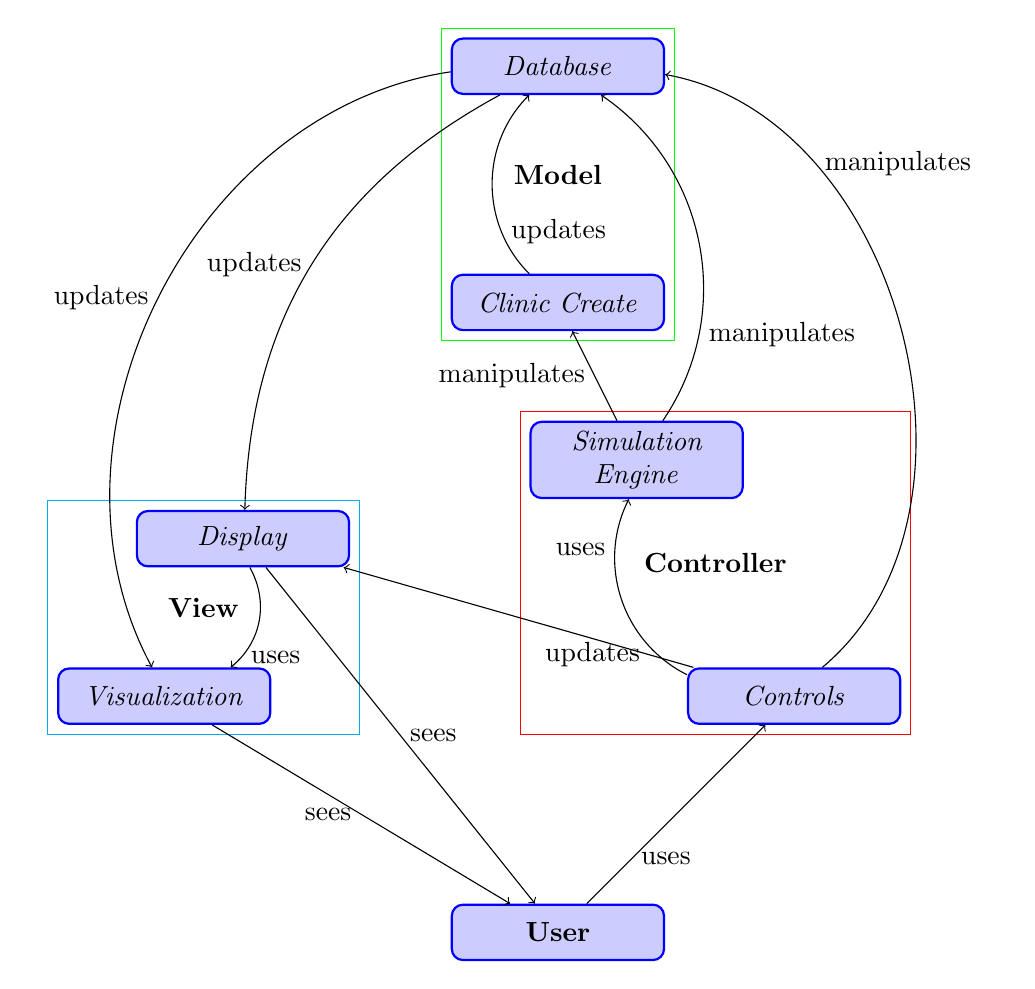
\begin{tikzpicture}
		[auto,
		block/.style ={rectangle, draw=blue, thick, fill=blue!20, text width=7em,align=center, rounded corners, minimum height=2em},
		line/.style ={draw, thick, -latex',shorten >=2pt},
		cloud/.style ={draw=red, thick, ellipse,fill=red!20,
		minimum height=1em},nodedec/.style={shape=circle,inner sep=2pt,draw,thick},
		arrowdec/.style={->}]	
		\draw (0,-2) node[block] (USER) {\textbf{User}};
		\path (3,1) node[block] (WEBGUI) {\textit{Controls}}
		      (1,4) node[block] (SIM) {\textit{Simulation Engine}}
		      (0,6) node[block] (CRE) {\textit{Clinic Create}}
		      (0,9) node[block] (DATA) {\textit{Database}}
		     (-4,3) node[block] (DIS) {\textit{Display}}
		     (-5,1) node[block] (VIS) {\textit{Visualization}}
		     ;
		
		\node[draw=red, fit=(WEBGUI) (SIM)](FIt1) {\textbf{Controller}};
		\node[draw=green, fit=(CRE) (DATA)](FIt2) {\textbf{Model}};
		\node[draw=cyan, fit=(DIS) (VIS)](FIt3) {\textbf{View}};
		
		\path
		(USER) edge[arrowdec] node[right,near start] {uses} (WEBGUI)
		(WEBGUI) edge[arrowdec,bend left=45] node[left,near end] {uses} (SIM)
		(SIM) edge[arrowdec] node[left] {manipulates} (CRE)
		(SIM) edge[arrowdec,bend right=45] node[right,near start] {manipulates} (DATA)
		(WEBGUI) edge[arrowdec,bend right=65] node[right,near end] {manipulates} (DATA)
		(CRE) edge[arrowdec, bend left = 45] node[right, near start] {updates} (DATA)
		(DATA) edge[arrowdec,bend right = 30] node[left] {updates} (DIS)
		(DATA) edge[arrowdec,bend right = 55] node[left] {updates} (VIS)
		(WEBGUI) edge[arrowdec] node[left, very near start] {updates} (DIS)
		(DIS) edge[arrowdec, bend left = 40] node[right, very near end] {uses} (VIS)
		(DIS) edge[arrowdec] node[right] {sees} (USER)
		(VIS) edge[arrowdec] node[left] {sees} (USER)
		;	
		\end{tikzpicture}
	\end{center}
	\caption{Breakdown of MVC Design} \label{MVC}
\end{figure} 
\newpage 
The \textbf{Controller} can be broken up into two primary components: \textit{Controls}, which represents the how the user interfaces with the product and \textit{Simulation Engine}, which manages and runs the clinic simulation. The \textbf{Model} also can be broken into two primary components: \textit{ClinicCreate}, which manipulates the database information into a form usable to \textit{Simulation Engine} and the \textit{Database}, which manages all data base operations. The \textbf{View} can be broken down into two major components: \textit{Display}, which handles the GUI for the website, and \textit{Visualization} which displays the simulation data to the users.

\subsection{Controls}
\textit{Controls} is a grouping of modules that are used by the user to interact with the system. They allow the user to enter input, issue commands to the simulation engine and change what is displayed by the view. It is primarily written in python 3 and uses the pymongo package to interact with MongoDB .\\
\textit{Controls} interacts with the \textit{Simulation Engine} and
\textit{Database} using the simengine() method. It also interacts with the display using the methods found in clinicflowx/views.py . \\
The component \textit{Controls} allows the system to fufill both functional and non-functional requirements. It controls the interaction between elements in the program, meaning it determines what is going to be run. It also must do so in a way that is satisfactory to the end user. \\
\subsection{Simulation Engine}
\textit{Simulation Engine} is a grouping of modules that are used by the program
to create and run the simulations for a clinic. It manipulates the data
from the \textit{Clinic Create} to create the simulation. It then is able to generate multiple simulations, and commit the results the to \textit{Database}. \textit{Simulation Engine} is primarily written in Python 3, and it uses the SimPy discrete event simulation package. \\
\textit{Simulation Engine} interacts with others modules through the method SimulationEngine.py . This method calls the other methods needed to run a simulation of the clinic. It takes as input: 
\begin{enumerate}
\item a dataset that represents the clinic's information
\item a dataset that represents the provider's schedule
\item a dataset that represents the patient's schedule
\item a target destination for the output data
\end{enumerate}
As output, it uses (or creates if it does not exist) a file containing all of the information generated by the simulation. It does this via AddSimResult.py . \\
The component \textit{Simulation Engine} exists primarily to fulfill the functional requirements, namely actually being able to create and record a simulation. It also addresses many of the nonfunctional requirements, such as simulation speed. \\
\subsubsection{Data Analysis}
\textit{Simulation Engine} also has to solve the problem of how we implemented a discrete event simulation to provide realitic results. 
To allow it to be able to do this, we had to do background research into the clinic, and do analysis on the clinic's existing data sets. \\
Plots were created to understand the types of underlying variance in each of the sections of the clinic, as well as the variance in arrival times. For arrival times, we investigated the distribution of the differences between the scheduled arrival times and the actual arrival times. 

\begin{figure}[H]
	\centering
	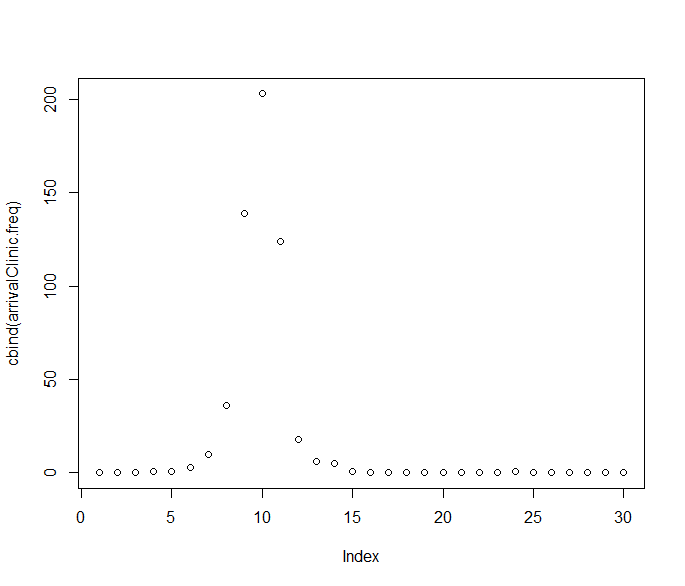
\includegraphics[width=8cm]{ScheduledVersusActual}
	\caption{A plot of the distribution of scheduled arrivals versus actual arrivals}
\end{figure}
The X-axis in the above figure is the "bin" in which each difference was placed. 10 represents no difference between scheduled and actual arrivals, with 0 being -30 minutes the largest difference. The Y-axis in the above figure is the frequency of which each of these bins occur. \\
The above figure tells us that most people arrive around the time when they are scheduled, and that the variance appears to be approximately normal( Gaussian). \\
Next we looked at the first class of modules, that have fairly standard service times. To get an idea of the variance in these service times, we looked at the difference between the start time of the module and the finish time. The following plot is for"Registration", a typical example of this type of module: \\
\begin{figure}[H]
	\centering
	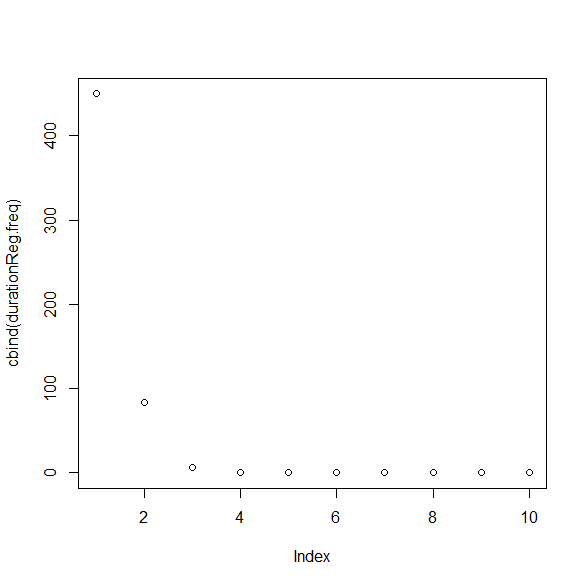
\includegraphics[width=8cm]{RegistrationVariance}
	\caption{A plot of the distribution of time spent in "Registration"}
\end{figure}
The X-axis in the above figure is the "bin" in which each time length is placed. 0 represents 0 to 3 minutes spent in the module, with each remaining bin representing another 0-3 minutes. The Y-axis in the above figure is the frequency of which each of these bins occur. \\
From the above figure, we can see that most patients finish these modules quickly and with a consistent service time. There are a few patients who take longer. This suggests that we should use an exponential model for the variance in this module. Other modules of this class show a similar variance distribution. \\
Finally we investigated another class of modules, which have a more extreme spread of variance in the service times. This is because these modules contain more complicated proceedures that have no standard service time. To get an idea of the variance in these service times, we looked at the difference between the start time of the module and the finish time. The following plot is for"XRayinRadiology", a typical example of this type of module: \\
\begin{figure}[H]
	\centering
	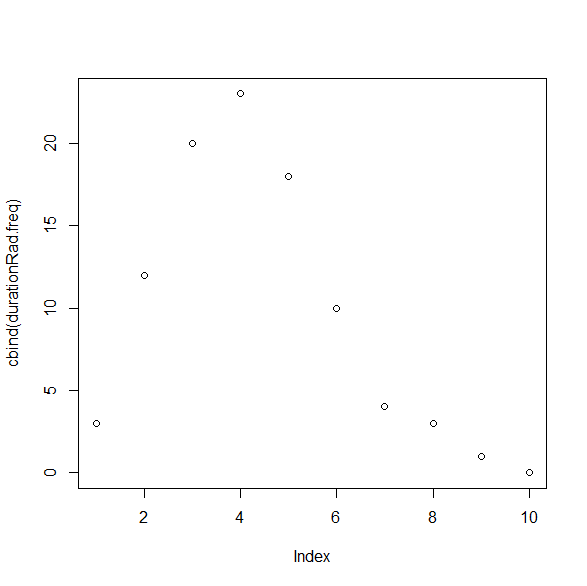
\includegraphics[width=8cm]{RadVariance}
	\caption{A plot of the distribution of time spent in "XRayinRadiology"}
\end{figure}
The X-axis in the above figure is the "bin" in which each time length is placed. 0 represents 0 to 3 minutes spent in the module, with each remaining bin representing another 0-3 minutes. The Y-axis in the above figure is the frequency of which each of these bins occur. \\
From the above figure, we can see that there is a large amount of variation between the amount of time any one patient would spend in this module. Some patients finish within 3 minutes, while most spend around 15 minutes. This suggests that we should try to model this variance with a different distribution, such as a normal (Gaussian) distribution. \\
In our implementation, we were able to take advantage of the results of this analysis to improve our models. We were able to use Python 3's libraries to generate random numbers as part of distributions built from the data sets we were provided on the clinic. We were also able to catergorize each module into one of two types (simple or complex). The variance of the arrival times was hard to model properly, so many method were tried before the final version used in the simulation engine was selected.
\subsection{Clinic Create}
\textit{Clinic Create} is a grouping of modules that take the data from the \textit{Database} and create useable files and tables for \textit{Simulation Engine}. It maintains some of the clinic information, and general rules. \textit{Clinic Create} is written in Python 3.\\
It takes input from other functions in the cliniccreate() method, and this method also provides files to \textit{Simulation Engine} to allow that module to function. \\
\textit{ClinicCreate} exists as a group of helpers for other methods. It does not solve any requirements itself, but it contributes to other modules being able to fulfill their requirements. \\
\subsection{Database}
\textit{Database} is a grouping of modules that manage the database functions. It manages the tables, and it able to create and modify existing data tables. \textit{Database} uses a  MongoDB NoSQL framework. \\
This is cluster of database creation and management functions. They exist primarily in ClinicMongoDB.py . It does not contain input and output functions, but it manages contructs that get used by other modules. \\
\subsection{Display}
\textit{Display} is a grouping of modules that manage the web display to the user. It displays the simulation results and information from \textit{Database}. It controls what the user sees. \textit{Display} is primarily written in Python 3, html and css. \\
It shows the html pages to the user. It also takes requests from \textit{Controls} to update and change the pages displayed. \\
\textit{Display} exists to fulfill the function requirements involving showing the user results. It also must fulfill many non-functional requirements related to usabaility. \\
\subsection{Visualization}
\textit{Visualization} is a grouping of modules that create
the visualizations of the data that are displayed to the users. 
It gets the data from \textit{Database} and give the visualizations to \textit{Display}. \textit{Visualization} was primarily written in ...

\section{Display: User Interface Design}
\subsection{Overview}


\begin{figure}[H]
	\centering
	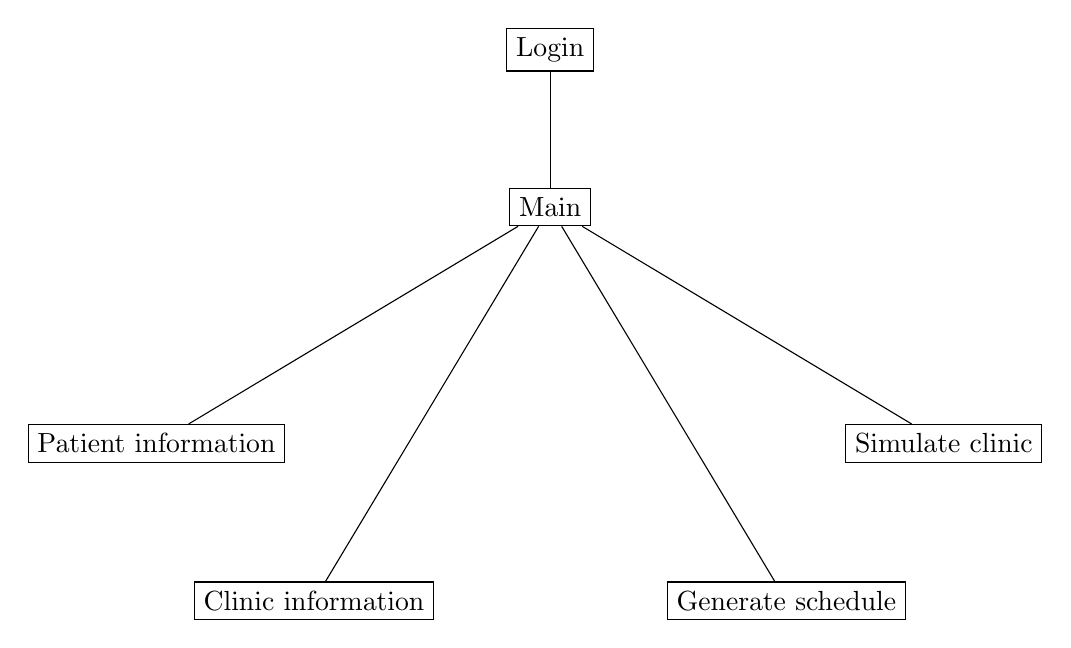
\begin{tikzpicture}
	% Design of Simulation Engine
	\node[draw] (LOG) at (0,5) {Login};
	\node[draw] (MAIN) at (0,3) {Main};
	\node[draw] (PI) at (-5,0) {Patient information};
	\node[draw] (SC) at (5,0) {Simulate clinic};
	\node[draw] (CI) at (-3,-2) {Clinic information};
	\node[draw] (GS) at (3,-2) {Generate schedule};
	
	\draw[-,draw=black] (MAIN) to (LOG);
	\draw[-,draw=black] (SC) to (MAIN);
	\draw[-,draw=black] (PI) to (MAIN);
	\draw[-,draw=black] (CI) to (MAIN);
	\draw[-,draw=black] (GS) to (MAIN);
	\end{tikzpicture}
	\caption{User Interface Design}
\end{figure}

\subsection{Navigation flow}
The first page presented to the user is the login page. The user must login as a manager or a authentic viewer before further operation. After logging in, the user will be redirected to the main menu page. The main menu page can direct user to the patient information page, clinic information page, generate schedule page and simulate schedule page. The user who log in as a viewer can only view patient information and generated schedules. Meanwhile the manager account would have viewer capabilities, in addition to being able to add/change patient information, add or change clinic attribute data, run simulations on specific patient data, or generate schedules based on patient data.

\noindent \newline
Each page has a navigation bar which let user transfer to different page. Each page has a logout button, thus the user can quit the system at any time. \\

\subsection{Login}
The user has to log in with the correct account and password before using the system. The login page has straight forward design which allows users to easily log in. This page contains internal validation to protect the system. This page can distinguish the user as a manager or a viewer, and gives the user corresponding authority. 

\subsection{Main Menu}
This page outlines general information such as today’s reservation schedule, today’s patients in list, and patients need schedule for next day which can give the user a quick overview. This page can guide the user to patient information,clinic information, clinic simulation, and schedule generation pages.

\subsection{Patient Information}
The manager account user can insert patient specific information such as name/id, appointment time, and required procedures into the system’s database. There is a list of empty fields for the user to fill up. The fields for appointment time and procedures are vital and must be entered in order to add the patient to the system, while other fields may be optional . The save button will validate the inputs before saving the patient data into database. The validation function will check the inputs to ensure the data consistency. If errors occur, the system will retain the inputs and inform the user of the source of error. Bulk patient data import is also supported through import of standardized csv files.

\noindent \newline
Both manager and view accounts are able to also see information on all patients current in the system. This will be presented both as list and timetable formats. Search and filter functionality will be included to allow users to target a particular subset of patients. Modification of existing records is also allowed, but only be the manager account.

\subsection{Clinic Information}
This page will give an overview of the attributes that model the clinic. This includes employee numbers, break times, starting times, etc. Both manager and view accounts will have access to this page, but only manager accounts will be able to edit the information therein and save it to the database. Multiple profiles for clinic information are also supported. This allows the user to simulate the clinic under models and compare the results.

\subsection{Simulate Clinic}
This page will be the interface to the simulation engine. The user will be able to run a simulation of the clinic given the data provided in the patient and clinic information sections of the application. The results of the current simulation and its summary statistics, as well as those of previous simulations, will be displayed here. The user is able to choose the day, and clinic data profile to use in the simulation. This page will also allow users to modify patient or clinic attributes (such as number of nurses available) to quickly see their effects on simulated clinic operation. 

\noindent \newline
While managers and viewers will both be able to see past results, only managers have the authority to run simulations.

\subsection{Generate Schedule}
This page allows users to generate optimized patient arrival schedules based on patient and clinic information data. Users can select the day and clinic profile to generate schedules for. Top results will be displayed with their summary statistics in an easily comparable format. Past generated schedules are also viewable, and sorted by the date. The schedule will clearly present the arrive time and patients’ first visit room.  Manager has the permission to delete or update existing schedules. The manager account user can add a patient’s reservation into the existed schedule. The backend system will simulate the procedure and time expense of the patient inside clinic. The system also will alert the use to any potential issues such as a patient having to wait too long.

\noindent \newline
While managers and viewers will both be able to view past generated schedules, only managers have the authority to generate new schedules.




\section{Simulation Engine}

\subsection{Design Description}
The simulation engine is the core component set which is responsible for running the simulation of the clinic. The patients and their associated data are the entities that are tracked by the simulation, the clinic workers are the available resources that can service the patients, while the clinic environment acts as the constraints under which the patients flow through the system. This lends itself to a natural tree like organization structure. The modules thus have low coupling and high cohesion, with details pertinent to their operation being compartmentalized. \textit{SimulationEngine} and Simulation run the simulation events, \textit{PatientSchedule},\textit{ HealthCareSchedule}, and \textit{Clinic} maintain the objects used in the simulation, while \textit{Patient}, \textit{HealthCareWorker}, and \textit{ClinicModule} keep track of the data if individual units in the simulation.

\subsection{Simpy}
Simpy is a Process-based discrete-event simulation framework which works with Python 3. It is well known and has a solid support base. The framework is relatively easy to work with and allows for a variety of event simulation types which are useful to this project. 

\begin{figure}[H]
\centering
    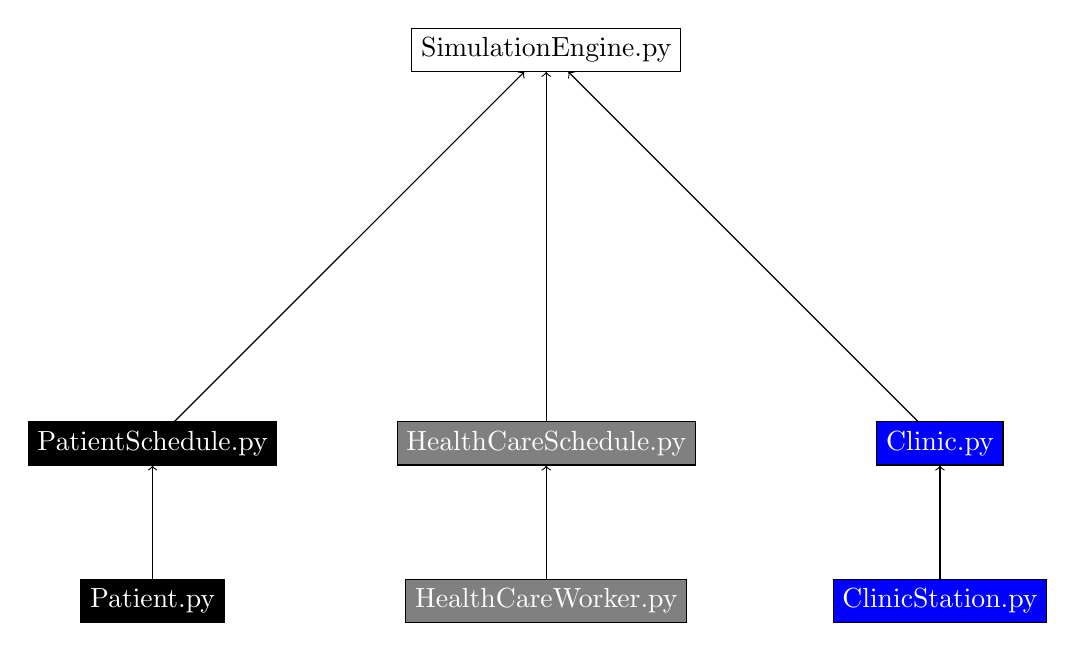
\begin{tikzpicture}
    % Design of Simulation Engine
    \node[draw] (SIM) at (0,5) {SimulationEngine.py};
    %\node[draw] (SIM) at (0,3) {Simulation.py};
    \node[draw,fill=black,text=white] (PSC) at (-5,0) {PatientSchedule.py};
    \node[draw,fill=gray,text=white] (HSC) at (0,0) {HealthCareSchedule.py};
    \node[draw,fill=blue,text=white] (CLI) at (5,0) {Clinic.py};
    \node[draw,fill=black,text=white] (PAT) at (-5,-2) {Patient.py};
    \node[draw,fill=gray,text=white] (HCW) at (0,-2) {HealthCareWorker.py};
    \node[draw,fill=blue,text=white] (CLM) at (5,-2) {ClinicStation.py};

   % \draw[->,draw=black] (SIM) to (SE);
    \draw[->,draw=black] (CLI) to (SIM);
    \draw[->,draw=black] (PSC) to (SIM);
    \draw[->,draw=black] (HSC) to (SIM);
    \draw[->,draw=black] (PAT) to (PSC);
    \draw[->,draw=black] (HCW) to (HSC);
    \draw[->,draw=black] (CLM) to (CLI);
   % \node at (0.0, -4.0) {\textit{ Figure 1: Simulation Engine Uses Diagram}};
    \end{tikzpicture}
    \caption{Simulation Engine Uses Diagram}
\end{figure}


\subsection{SimulationEngine.py}
\subsubsection{SimulationEngine(clinicFile,employeeFile,patientFile,outFile)}
\begin{itemize}  
\item Acts as a top level for the program
\item Handles File I/O for simulation
\item Uses HealthCareSchedule, PatientSchedule and Clinic tables
\item Calls the simulation function
\item It helps meet the following requirements:
%\item Manages the simulation of the clinic
%\item Uses SimPy
%\item Has methods for workerRun and patientRun to create "threads" for the objects
%\item Also contains the simulation resources
%\item Uses HealthCareSchedule, PatientSchedule and Clinic
\end{itemize}
\subsubsection{Simulation(env,clinic,workerSchedule,patientSchedule,outfile)}
\begin{itemize}
	\item Manages the simulation of the clinic
	\item Uses SimPy to run a discrete event simulation
	\item Is called by SimulationEngine(), and uses workerRun() and patientRun() to create the simulation
	\item This function also handles the data analysis for the simulation results
	\item It helps meet the functional requirements related to the simulation:
\end{itemize}
\subsubsection{workerRun(env,worker,clinic,resources)}
\begin{itemize}
	\item Is the function that represents the "logic" that the worker threads follow
	\item Is used by Simulation to simulate the health care providers
	\item It helps meet the functional requirements related to the workers:
	It helps the simulation be realisitic
\end{itemize}
\subsubsection{patientRun(env, patient,clinic,resources)}
\begin{itemize}
	\item Is the function that represents the "logic" that the patient threads follow
	\item Is used by Simulation to simulate the patients
	\item It helps meet the functional requirements related to the patients:
	It helps the simulation be realisitic
\end{itemize}

\subsection{Clinic.py}
\begin{itemize}  
\item Contains the information about the clinic
\item Constructor method reads in clinic data from file
\item Uses ClinicStation
\end{itemize}

\subsection{ClinicStation.py}
\begin{itemize}  
\item Contains information about an individual station in the clinic
\item Contains methods for activating and deactivating a station
\item Contains a method for getting a random number, generated from that particular station randomness
\end{itemize}

\subsection{HealthCareSchedule.py}
\begin{itemize}  
\item Contains information about the provider's schedule in the clinic
\item Contains methods for generating a schedule and for reading a schedule from a file
\item Uses HealthCareWorker.py
\end{itemize}

\subsection{HealthCareWorker.py}
\begin{itemize}  
\item Contains information about a particular provider in the clinic
\item Contains methods to change the worker's scheduled times, and which station they are at
\item Has a toString method for ease of use
\end{itemize}

\subsection{PatientSchedule.py}
\begin{itemize}  
\item Contains information about the patient's schedule in the clinic
\item Contains methods for generating a schedule and for reading a schedule from a file
\item Uses Patient.py
\end{itemize}

\subsection{Patient.py}
\begin{itemize}  
\item Contains information about a patient in the clinic
\item Has methods to adjust the patient's schedule, and help keep track of their actions throughout the clinic
\item Has a toString method for ease of use
\end{itemize}




\section{Database Structure}

\subsection{Implementation Details}
MongoDB will be used as a database to store all input data related to modeling the clinic, as well as output data generated from simulation. The database will also be used to recall previously stored data. MongoDB does not have a rigid structure, but its simplicity is well suited for this project. All data sets will be stored in a corresponding MongoDB collection. All data has a key attribute to improve searching efficiency and avoid duplication.

\subsection{Data format}
The \textbf{patient} collection contains all required patient information. This includes patient name/id, appointment date, time, as well as the list of services required by the patient. This information will be used to simulate clinic operations on a per day basis.
\begin{table}[H]
\centering
\caption{Patient Table}
\label{patient-table}
\begin{tabular}{|l|l|}
\hline
Attribute Name   & Sample Value                \\ \hline
Patient Name     & Jack Square                 \\ \hline
Reservation Date & 2017-01-01                  \\ \hline
Reservation Time & 8:15                        \\ \hline
Procedure        & Interview, Bloodwork, x-ray \\ \hline
\end{tabular}
\end{table}
\hfill

The \textbf{clinic} collection contains all attributes of the clinic we are modeling. This data will act as constraints on the clinic simulation, and can be modified by staff to accommodate operational changes.
\begin{table}[H]
\centering
\caption{Clinic Table}
\label{clinic-table}
\begin{tabular}{|l|l|}
\hline
Attribute Name           & Sample Value \\ \hline
Nurse Number             & 3            \\ \hline
Available Interview Room & 3            \\ \hline
Clinic Open Time         & 8:00         \\ \hline
Clinic Close Time        & 18:00        \\ \hline
Reception Close Time     & 15:00        \\ \hline
\end{tabular}
\end{table}

The \textbf{result} collection contains all results from the simulations once they complete. This data will be used directly by the staff to help in deciding patient flow within the clinic during operation. This data will also help inform staff of attribute or scheduling effects on clinic operations.
\begin{table}[H]
\centering
\caption{Results Table}
\label{result-table}
\begin{tabular}{|l|l|}
\hline
Attribute Name         & Sample Value \\ \hline
Day                    & 2017-01-01   \\ \hline
Simulation Run \#      & 1            \\ \hline
AVG duration bloodwork & 20 minutes   \\ \hline
AVG patient wait time  & 1 hr         \\ \hline
Final patient end time & 17:00        \\ \hline
\end{tabular}
\end{table}
\hfill

\subsection{Sanitation}
Simulation engine relies on the format and accuracy of data. The patterns of data must match the pattern inside simulation engine to ensure the simulation engine runs properly. Upon insertion or modification of data, a validation process verifies the inputs or changes before storing into database. Invalid inputs or changes would be rejected and the system would inform the reason for rejection. If no error in input or changes is detected, the system should allow the updates. 


\section{Web Application Design}

\subsection{Frameworks}
The Django framework is used in this project. It provides the users with a way to access the simulation engine, which includes import data, running the simulation and utilizing other functions, and presents the simulation results in a concise and clear manner. At the same time, It helps to organize the backend structure of the project, even though it also supports the front end user interface. The following is a breakdown of the framework as it applies to our project.

\begin{itemize}  
\item models.py: 
integrates the simulation engine. It also deals with data flow from database to the simulation engine, and sends the corresponding outputs of the engine to the views.py. Other modules may be required to interact with the MongoDB as a database interface.
\item views.py, static folder and templates folder: 
when the users send requests to the presetting URL address, it acts as a router and directs the users to pages that are generated from the template html in the templates folder. Since the static template HTML will be merged into the simulation results by a dynamic mechanism, the users can view the simulation results and operate the simulation engine instantly.
\item test.py: 
for the later testing cases, it ensures the backend works correctly and meets the design requirements.
\item  urls.py: 
stores the settings of the URL address for users to visit.
\end{itemize}


\end{document}
